\begin{frame}
  \frametitle{\problemtitle}
  \begin{block}{Problem}
  	Given the height field representing a wall, decide if you can add $2\times1$ blocks to create a wall of width exactly~$w$ and height exactly $h$.
  \end{block}
  \begin{center}
  	\includegraphics[width=0.33\textwidth]{sample}
  \end{center}
  \pause
  \begin{block}{Solution\only<3>{?}}
  	\begin{itemize}
  		\item Given a subgraph of a $w \times h$ grid graph, decide if it has a perfect matching
  		\item Since the graph is a grid i.e.\ bipartite this can be done in $w\cdot h\cdot \sqrt{w\cdot h}$
  		\pause
  		\item [$\Rightarrow$] This is much too slow
  	\end{itemize}
  \end{block}
\end{frame}

\tikzset{
	visible on/.code={%
		\ifthenelse{\equal{#1}{}}{%
			\tikzset{alt={<\value{beamerpauses}->{}{opacity=0}}}%
		}{%
			\tikzset{alt={#1{}{opacity=0}}}%
		}%
	},%
	alt/.code args={<#1>#2#3}{%
		\alt<#1>{\pgfkeysalso{#2}}{\pgfkeysalso{#3}}%
	}%
}

\definecolor{red}{HTML}{972e21}
\definecolor{yellow}{HTML}{ebb83f}
\definecolor{blue}{HTML}{7999db}

\begin{frame}
	\frametitle{\problemtitle}
	\begin{center}		
		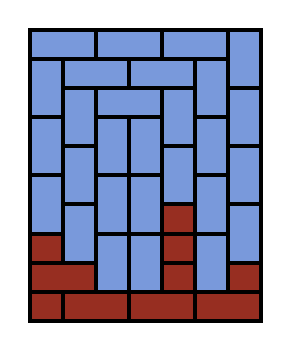
\begin{tikzpicture}[x=0.42cm,y=0.37cm,line width=0.05cm]
			\draw (0,0) rectangle(7,10);
			
			\draw[fill=red] (0,2) rectangle(1,3);
			\draw[fill=red] (0,1) rectangle(2,2);
			\draw[fill=red] (0,0) rectangle(1,1);
			\draw[fill=red] (1,0) rectangle(3,1);
			
			\draw[fill=red] (3,0) rectangle(5,1);
			\draw[fill=red] (4,1) rectangle(5,2);
			\draw[fill=red] (4,2) rectangle(5,3);
			\draw[fill=red] (4,3) rectangle(5,4);
			\draw[fill=red] (5,0) rectangle(7,1);		
			\draw[fill=red] (6,1) rectangle(7,2);
			
			
			\draw[fill=blue,visible on=<2->] (0,3) rectangle(1,5);
			\draw[fill=blue,visible on=<2->] (0,5) rectangle(1,7);
			\draw[fill=blue,visible on=<2->] (0,7) rectangle(1,9);
			\draw[fill=blue,visible on=<3->] (0,9) rectangle(2,10);
			
			
			\draw[fill=blue,visible on=<4->] (1,2) rectangle(2,4);
			\draw[fill=blue,visible on=<4->] (1,4) rectangle(2,6);
			\draw[fill=blue,visible on=<4->] (1,6) rectangle(2,8);
			\draw[fill=blue,visible on=<5->] (1,8) rectangle(3,9);
			
			
			\draw[fill=blue,visible on=<6->] (2,1) rectangle(3,3);
			\draw[fill=blue,visible on=<6->] (2,3) rectangle(3,5);
			\draw[fill=blue,visible on=<6->] (2,5) rectangle(3,7);
			\draw[fill=blue,visible on=<7->] (2,7) rectangle(4,8);
			\draw[fill=blue,visible on=<7->] (2,9) rectangle(4,10);
			
			
			\draw[fill=blue,visible on=<8->] (3,1) rectangle(4,3);
			\draw[fill=blue,visible on=<8->] (3,3) rectangle(4,5);
			\draw[fill=blue,visible on=<8->] (3,5) rectangle(4,7);
			\draw[fill=blue,visible on=<9->] (3,8) rectangle(5,9);
			
			
			\draw[fill=blue,visible on=<10->] (4,4) rectangle(5,6);
			\draw[fill=blue,visible on=<10->] (4,6) rectangle(5,8);
			\draw[fill=blue,visible on=<11->] (4,9) rectangle(6,10);
			
			
			\draw[fill=blue,visible on=<12->] (5,1) rectangle(6,3);
			\draw[fill=blue,visible on=<12->] (5,3) rectangle(6,5);
			\draw[fill=blue,visible on=<12->] (5,5) rectangle(6,7);
			\draw[fill=blue,visible on=<12->] (5,7) rectangle(6,9);
			
			
			\draw[fill=blue,visible on=<13->] (6,2) rectangle(7,4);
			\draw[fill=blue,visible on=<13->] (6,4) rectangle(7,6);
			\draw[fill=blue,visible on=<13->] (6,6) rectangle(7,8);
			\draw[fill=blue,visible on=<13->] (6,8) rectangle(7,10);
		\end{tikzpicture}
	\end{center}
	\begin{block}{Solution}
		\begin{itemize}
			\item There is a greedy strategy which finds a perfect matching if one exists
			\pause
			\begin{itemize}
				\item Go from left to right
				\item Place as many $1\times 2$ blocks from the bottom to the top as fit in the current column
				\item If needed place $2\times 1$ blocks on the top which go into the next column 
			\end{itemize}
			\pause[14]
			\item To simulate this efficiently, only store the height of the lowest brick coming from the left%
			\item This value either increases or decreases by $1$ if we go to the next column
		\end{itemize}
	\end{block}
\end{frame}
